\section{Métodos e Materiais}
    Para realização deste trabalho, foram utilizados os seguintes dispositivos:
    \subsection{Forno de Convecção Miniconv}
        O forno para controle da temperatura é o Miniconv, da empresa PRÁTICA KLIMAQUIP IND. E COM. S/A, ilustrado na Figura ~\ref{fig:Forno}, o qual utiliza convecção de circulação de ar por turbina. Esse modelo de forno é monofásico com tensão de alimentação de $220 \ [V]$ e potência de $2,56 \ [kW]$ \cite{Manual_Miniconv}.
        \begin{figure}[H]
            \centering
            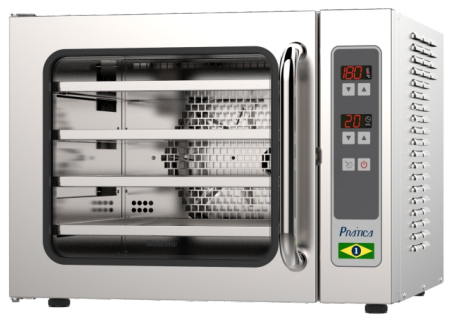
\includegraphics[width=0.48\textwidth]{Figuras/FornoMiniconv.png}
            \caption{Forno Miniconv, da empresa PRÁTICA \cite{Manual_Miniconv}.} \label{fig:Forno}
        \end{figure}
    \subsection{S7-1200 e TIA Portal}
        Para leitura dos dados de entrada, acionamento dos dispositivos de saída e desenvolvimento da lógica de controle, foi utilizado o CLP S7$-$1200 1214C DC/DC/DC da Siemens, com a CPU 6ES7 214-1AG40-0XB0, ilustrado na Figura ~\ref{fig:PLC_Siemens}. O CLP é compacto com $100$ KB de memória de programa e possui 14 entradas digitais de $24$ VDC, 10 saídas digitais $24$ VDC, 2 entradas analógicas $0-10$ VDC \cite{CLP_S7-1200}. A entrada analógica receberá o sinal proveniente da leitura do sensor de temperatura, enquanto as saídas digitais são responsáveis por ligar a resistência.
        \begin{figure}[H]
            \centering
                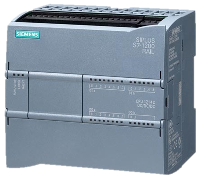
\includegraphics[width=0.35\textwidth]{Figuras/PLC.png}
                \caption{CPU 6ES7 214-1AG40-0XB0 $-$ Siemens \cite{CLP_S7-1200}.} \label{fig:PLC_Siemens}
        \end{figure}
        
        Como interface de programação para os controladores da Siemens, o TIA Portal (\textit{Totally Integrated Automation} - Automação Totalmente Integrada), permite aos usuários realizar tarefas de automação e acionamento de forma rápida e intuitiva usando configurações eficientes. A arquitetura do \textit{software} é projetada para alta eficiência e facilidade de uso, além de ser adequada para usuários novos e experientes \cite{TIA_Portal}.
        
        A interface possibilita programação através de linguagens de alto nível e apresenta as linguagens padronizadas pela norma IEC 61131 de acordo com as diferentes versões disponíveis. No projeto, é possível elaborar uma Interface Homem-Máquina (IHM) e desenvolver o programa de forma estruturada, organizado em pastas e em blocos de programação.
        
        Para desenvolvimento deste projeto, foi utilizada a versão V15 com as linguagens de programação ST \textit{(Structured Text)} $-$ Texto Estruturado, e LD (Ladder).  ~\ref{fig:PLC_Siemens}.
    \subsection{Relé de Estado Sólido com Cruzamento Zero}
        Os Relés de Estado Sólido com cruzamento zero são dispositivos utilizados para controlar elementos em corrente alternada (CA) que necessitam ser acionados quando a tensão é próxima, ou igual, a $0$. As cargas resistivas, como, por exemplo, a resistência de aquecimento, devem ser alimentadas com uma tensão de $0 \ [V]$ aumentada gradualmente para diminuir as chances de danificar o elemento.
        
        Considerando que durante os experimentos ocorrem comutações da carga em certos valores, o Relé de Cruzamento Zero atua com uma histerese de proteção \cite{Rele_EstadoSolido}, aumentando a vida útil do atuador. Na Figura ~\ref{fig:rele0cross} é possível observar o comportamento do relé, em que o tempo ativado se dá pelo semi ciclo hachurado:
        \begin{figure}[H]
            \centering
            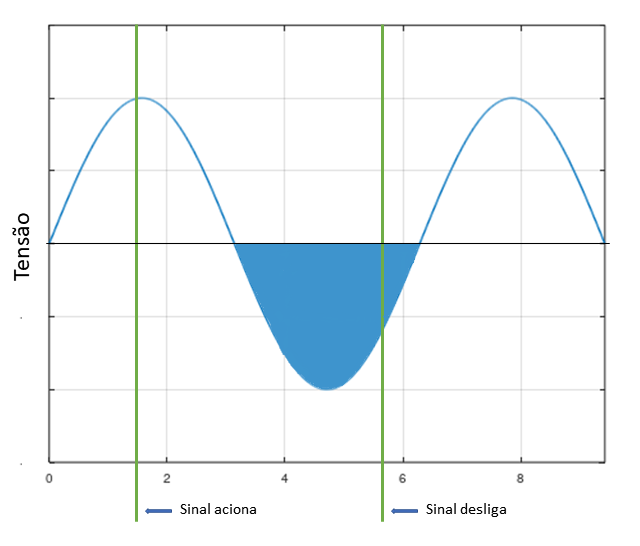
\includegraphics[width=0.48\textwidth]{Figuras/Rele0cross.png}
            \caption{Comportamento do Relé de Cruzamento Zero.} \label{fig:rele0cross}
        \end{figure}
        Quando o sinal de controle é aplicado, o relé observa a forma de onda da alimentação e aguarda até que o meio ciclo finalize para acionar a resistência.
    \subsection{Sensor e transmissor de temperatura}
        Como elemento sensor e dispositivo para medição da temperatura do forno, utilizou-se um Termopar Tipo J, ilustrado na Figura ~\ref{fig:TermoparJ}, cuja temperatura medida varia de $0 \ [^{\circ}C]$ até $760 \ [^{\circ}C]$:
        \begin{figure}[H]
            \centering
                %\includegraphics[width=0.35\textwidth]{Figuras/}
                \caption{Termopar Tipo J.} \label{fig:TermoparJ}
        \end{figure}
        
        O sensor realiza a leitura da temperatura da câmara do forno, que atinge no máximo $220 \ [^{\circ}C]$, desconsiderando o \textit{overshoot} possível, e fornece uma tensão proporcional ao valor medido, de acordo com o gráfico da Figura ~\ref{fig:GraficoTermopar}:
        \begin{figure}[H]
            \centering
                \includegraphics[width=0.48\textwidth]{Figuras/TermoparJ.jpg}
                \caption{Tensão $vs$ Temperatura no Termopar J} \label{fig:GraficoTermopar}
        \end{figure}
        
        Pelo gráfico, nota-se que a tensão de saída do Termopar J é baixa e pouco adequada para ser corretamente interpretada  na entrada analógica do CLP, na faixa $0$ a $10 \ [V]$. O ajuste da leitura do termopar utiliza um transmissor de temperatura, o qual fornece um sinal padronizado de corrente, de $4$ a $20$ mA, proporcional a temperatura do forno. Como a entrada analógica do CLP aceita valores de tensão, é considerado um resistor de $250 \ [\Omega]$ em paralelo com a saída do transmissor, fornecendo valores na faixa de $1$ a $5 \ [V]$ para a entrada analógica do CLP.

\subsection{Resistência de aquecimento}

A resistência é o componente responsável por aquecer a câmara do forno. Será utilizada como o elemento a ser controlado, onde seu funcionamento é comandado pelo PLC de acordo com o sistema de controle utilizado.
Possui comportamento resistivo e será acionada com o auxilio do relé de cruzamento 0.

    \subsection{Controle Liga/Desliga (On/Off)}
        O controle de duas posições, ou simplesmente controle \textit{On/Off}, é definido por um sistema em que, na maioria das aplicações, o atuador possui apenas dois estados ligado (\textit{On}) ou desligado (\textit{Off}). Dessa forma, o elemento atuador é considerado digital, pois apresenta apenas esses dois estados. Por ser um sistema simples e barato, é muito utilizado em controles domésticos e industriais \cite{Fundamentos_SistemasControle}.
            
        Considerando um sistema genérico, em que $u(t)$ é a saída do controlador e $e(t)$, o erro atuante, no controle de duas posições $u(t)$ assume o valor máximo ou mínimo de acordo com a polaridade de $e(t)$. A Equação ~\ref{eq:ControleOnOff} descreve o comportamento da saída do sistema, em que $U_1$ e $U_2$ são constantes \cite{Livro_Ogata}:
        \begin{equation}
            \label{eq:ControleOnOff}
            \begin{gathered}
                u(t) = U_1, \ para \ \ e(t) > 0 \\
                u(t) = U_2, \ para \ \ e(t) < 0
            \end{gathered}
        \end{equation}
        
        O controle do sistema se baseia na varição do \textit{Duty Cycle (DC)} do atuador, ou seja, na relação entre o tempo de sistema ligado $T_{ON}$ e o período do sinal $T = T_{ON}+T_{OFF}$, segundo a Equação ~\ref{eq:DutyCycle}:
        \begin{equation}
            \label{eq:DutyCycle}
            DC \ [\%]=\dfrac{T_{ON}}{T_{ON}+T_{OFF}}\cdot100=\dfrac{T_{ON}}{T}\cdot100
        \end{equation}
        
        Em valores percentuais, o \textit{Duty Cycle} caracteriza um valor médio de tensão contínua. Dessa forma, quanto mais tempo o sinal permanecer em nível lógico alto dentro de um período maior será a potência da resistência.
        \begin{figure}[H]
            \centering
            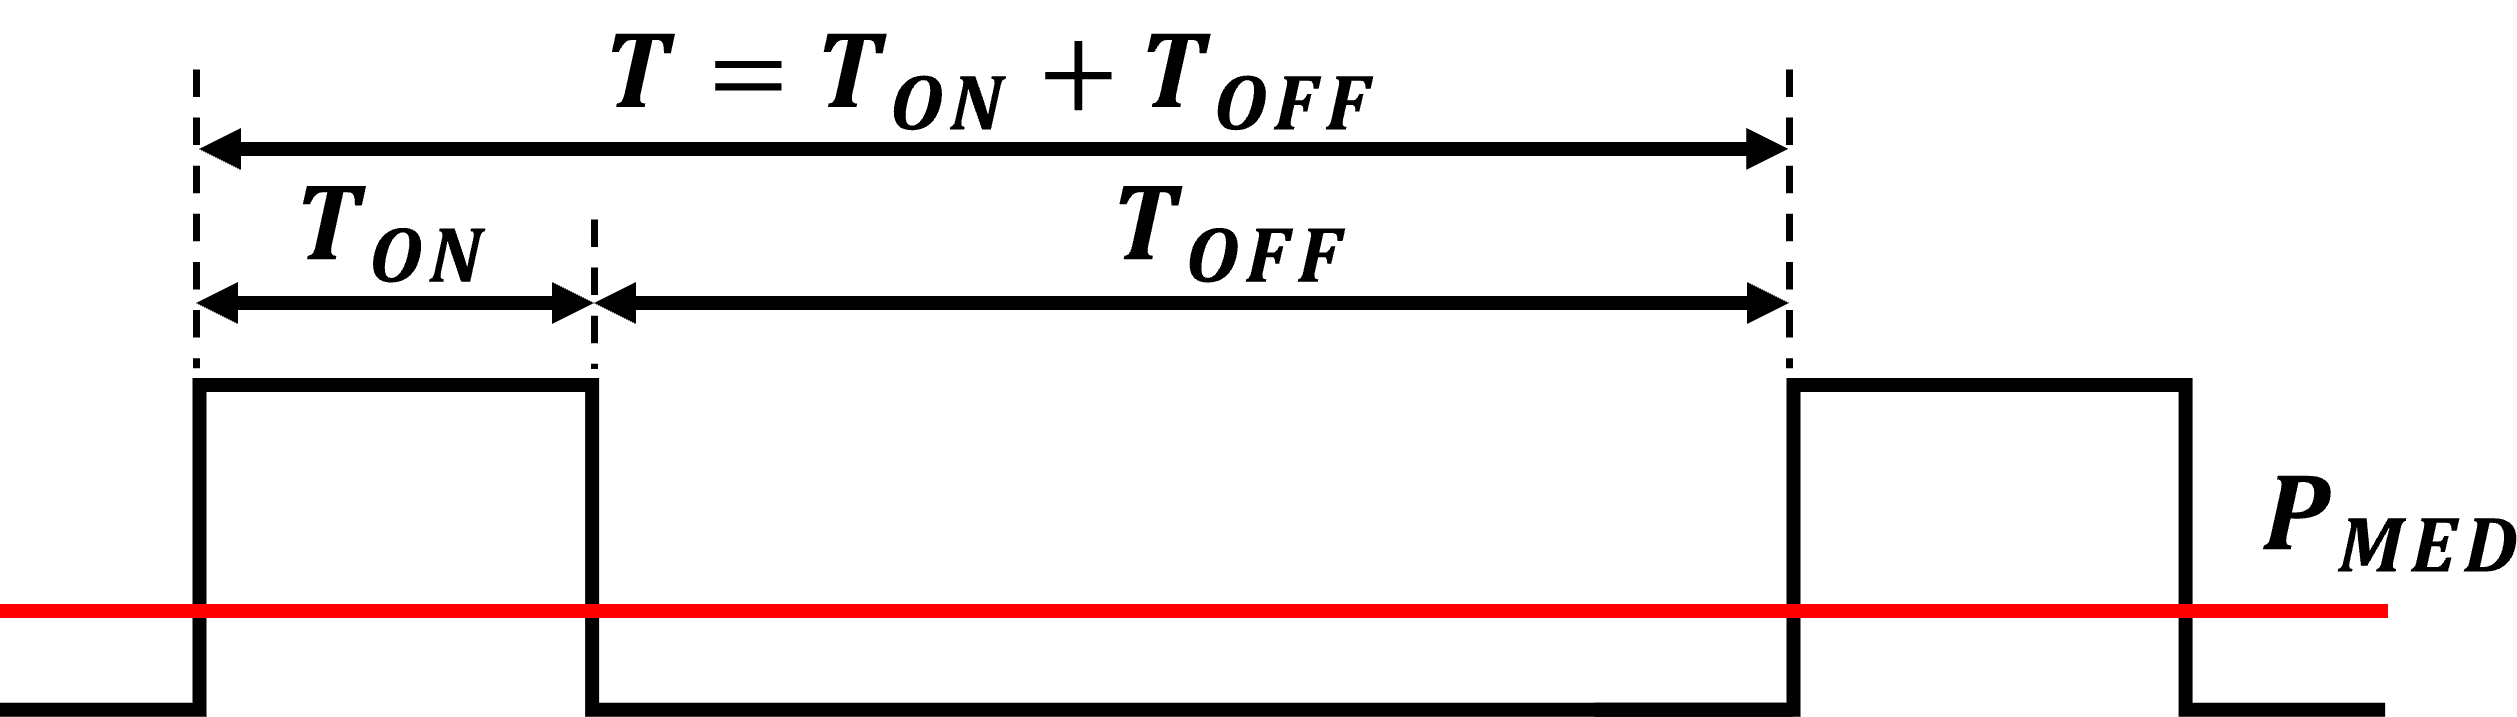
\includegraphics[width=0.48\textwidth]{Figuras/DutyCycle.png}
            \caption{Potência média da resistência.} \label{fig:DuteCycle}
        \end{figure}
        
        Na Figura ~\ref{FiguraOnOff}, é possível observar o comportamento da saída do sistema. Alguns modelos utilizam um intervalo diferencial para permitir uma lacuna em que o valor atual na saída não seja alterado com alto ciclo de comutação, permitindo, assim, que atuadores mecânicos ou eletrônicos tenham maior vida útil.
        \begin{figure}[H]
          \centering
          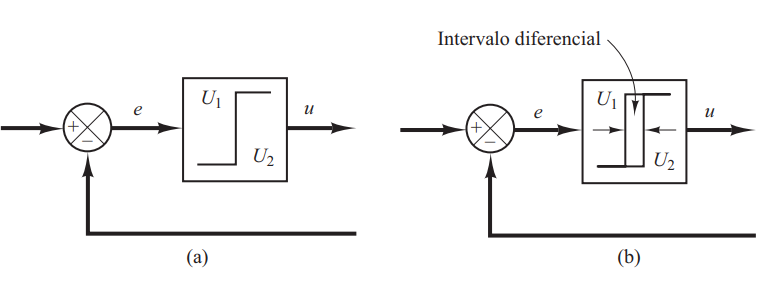
\includegraphics[width=0.48\textwidth]{Figuras/ControladorOnOff.png}
          \caption{Resposta típica de Sistemas com Controle \textit{On/Off}.} \label{FiguraOnOff} 
        \end{figure}
        
        Em decorrência do ciclo de comutação do atuador, o controle \textit{On/Off} tolera uma variação da amplitude da saída em relação ao \SetPoint \ em sistemas mais lentos ou com tempo morto. Dessa forma, torna-se evidente que, na maioria das aplicações, haverá erro atuante no processo, ou seja, $e(t) \neq 0$.
\subsection{Controle Proporcional/Integral/Derivativo - PID}
O controlador PID é amplamente usado em processos industriais, pois possui uma estrutura relativamente simples, mas suficiente para o uso em inúmeros processos. Trata-se de um algoritmo de controle composto por três partes $-$ proporcional, integral e derivativa, descritas a seguir:

\begin{itemize}
    \item Controle Proporcional (P): para um sistema com ação de controle proporcional, a função de transferência é modelada por um fator de ganho $K_P$. Na prática, esse ganho é, essencialmente, um amplificador ajustável que estabelece uma relação entre a saída e a entrada (erro $e(t)$), segundo a Equação ~\ref{eq:ControleP}:
         \begin{equation}
            \label{eq:ControleP}
            u(t) = K_P \cdot e(t) \ \rightarrow \ G_1(s) = \dfrac{U(s)}{E(s)} = K_P 
        \end{equation}
    A ação de controle proporcional reduz o tempo de resposta do sistema (tempo de subida $- \ t_r$) quando comparado a um controle simples do tipo \textit{On/Off}. Comumente, valores mais elevados de ganho proporcional aumentam a precisão do sistema em malha fechada, reduzindo, sem eliminar, o erro em regime permanente.
       
    \item Controle Integral (I): a ação de controle integral promove melhoria na precisão do sistema em regime permanente, pois elimina o erro, $e(t)=0$. Em contrapartida, o sistema pode tornar-se mais lento e aumentar o máximo pico da resposta para uma entrada do tipo degrau. A saída é modificada a uma taxa de variação proporcional à integral do erro, e pode ser definida em função de um ganho $K_I$ ou de um tempo de integral $T_I$, segundo a Equação ~\ref{eq:ControleI}:
    \begin{equation}
        \label{eq:ControleI}
        \centering
        \begin{gathered}
            u(t) = K_I \int  e(t) \ dt \\
            G_2(s) = \dfrac{U(s)}{E(s)} = \frac{K_I}{s} = \dfrac{K_P}{T_I \cdot s}
        \end{gathered}
    \end{equation}
    Analisando a função de transferência do controle integral, é notória a presença de um polo na origem do plano \textit{s}, caracterizando um sistema do tipo $1$. A partir do instante em que o erro se anula, o sinal de controle mantém um valor constante, o que significa obter, no sistema em malha fechada, uma referência constante com erro nulo em regime permanente \cite{Enciclopedia_Automatica}.
        
    \item Controle Derivativo (D): a ação derivativa é dita como antecipatória, pois o sistema responde a uma taxa de variação do erro e pode produzir uma correção significativa antes que o valor se torne muito elevado. O controle pode ser definido por um ganho $K_D$ ou por um tempo de derivada $T_D$, segundo a Equação ~\ref{eq:ControleD}, e pode melhorar o tempo de resposta do sistema: 
    \begin{equation}
        \label{eq:ControleD}
        \centering
        \begin{gathered}
            u(t) = K_D \cdot \dfrac{d}{dt}e(t) \\
            G_3(s) = \dfrac{U(s)}{E(s)} = K_D = K_P \cdot T_D \cdot s
        \end{gathered}
    \end{equation}
    Quando acrescentada a um controlador proporcional, a ação derivativa permite a obter um controlador de alta sensibilidade e estabilidade, entretanto só apresenta influência no regime  transitório, uma vez que um sinal estabilizado, em regime permanente, possui erro constante cuja derivada é $0$. A partir desse momento, apenas a parcela proporcional do controle tem atuação \cite{TCC_Controle1}.
\end{itemize}

A técnica de controle PID resulta da união dos efeitos descritos, em que a função de transferência $G(s)$ do sistema é modelada pela Equação ~\ref{eq:FuncaoPID}:
\begin{equation}
    \begin{gathered}
        \label{eq:FuncaoPID}
        G(s) = G_1(s) + G_2(s) + G_3(s) \\
        G(s) = K_P + \dfrac{K_I}{s} + K_D s = K_P \cdot \left (1 + \dfrac{1}{T_I s} + T_D s\right) 
    \end{gathered}
\end{equation}

O desempenho do sistema de controle em malha fechada em função dos ganhos é mostrado na Tabela ~\ref{EfeitosPID}:
    
\begin{table}[H]
    \centering  
    \caption{Comparação entre os efeitos do controle PID.} \label{EfeitosPID}
    \begin{tabular}{cccc} \cline{2-4}
         \rule{0mm}{4mm} & $K_P$ & $K_I$ & $K_D$ \\ \hline
         \rule{0mm}{4mm} Tempo de & \multirow{2}{*}{Reduz} & \multirow{2}{*}{Reduz} & Pouco \\
         subida &&& efeito \\ \hline
         \rule{0mm}{4mm} Máximo & \multirow{2}{*}{Aumenta} & \multirow{2}{*}{Aumenta} & \multirow{2}{*}{Reduz} \\
         pico &&& \\ \hline
         \rule{0mm}{4mm} Tempo de & Pouco & \multirow{2}{*}{Aumenta} & \multirow{2}{*}{Reduz} \\
         acomodação & efeito && \\ \hline
         \rule{0mm}{4mm} Erro regime & \multirow{2}{*}{Reduz} & \multirow{2}{*}{Elimina} & \multirow{2}{*}{Não muda} \\
         permanente &&& \\ \hline
    \end{tabular}
\end{table}

Na prática, o efeito ideal para o sistema de controle baseado em PID ocorre pelo cálculo correto dos valores dos ganhos $K_P$, $K_I$ e $K_D$ ou dos tempos $T_I$ e $T_D$. Esta etapa, enunciada como sintonia do controlador PID, leva em consideração os critérios de desempenho desejados para o sistema controlado. Trata-se de um passo realizado em consonância com as especificações de controle relacionadas ao \SetPoint \ ou à perturbação \cite{Sintonia_Visioli}.

Considerando que a resposta típica para um sistema com Controle PID respeita um sistema de segunda ordem, um sistema mal sintonizado pode elevar o \textit{overshoot} da saída. Analisando o comportamento do forno e sua aplicação no cozimento de alimentos, tal comportamento não é desejado. Dessa forma, a fim de reduzir o máximo pico e aumentar a estabilidade do sistema, pressupõe-se que o sistema controlado será lento.

\subsection{Controle por Lógica Difusa}
A lógica difusa consiste na representação de modelos com graus de incerteza ou imprecisão, permitindo o desenvolvimento de sistemas mais próximos ao raciocínio humano \cite{Resumo_Fuzzy}. Diferentemente da lógica do controle \textit{On/Off}, em que o atuador possui apenas dois estados (ligado ou desligado), na Lógica \Fuzzy \ um elemento pode pertencer parcialmente a um conjunto, definindo algumas regiões para a saída do sistema e criando transições mais flexíveis entre elas, enquanto no controle \textit{On/Off} as fronteiras são bem definidas.

O controle por Lógica \Fuzzy \ atribui à saída do sistema um valor resultante de uma função denominada grau de pertinência, definida por $\mu_{(x)}$, que indica o quanto cada elemento pertence ao conjunto. O retorno da função é um valor no intervalo $[0,1]$, ou seja, a saída pode variar em qualquer situação entre os estados “totalmente verdadeiro (1)” e “totalmente falso (0)” \ \cite{LivroFuzzy}, podendo pertencer a múltiplos grupos com diferentes graus de pertinência. As funções de pertinência de um sistema \Fuzzy \ podem se apresentar de vários tipos, sendo as funções triangular, trapezoidal e gaussiana as mais comuns.

A premissa inicial de um sistema por lógica \Fuzzy \ é definir quais serão as regiões para o dispositivo atuador. No caso do forno de convecção forçada, serão definidos cinco níveis de potência para o atuador, sendo que, quanto mais alta a potência, mais calor a resistência gera na câmara de cocção: Muito Baixa (MB), Baixa (B), Média (M), Alta (A) e Muito Alta (MA). 

A potência da resistência será MA quando $e(t) \gg 0$, diminuindo a potência à medida que o erro diminiu ou se torna negativo. A resistência terá uma potência média caso a temperatura esteja estabilizada próxima ao \SetPoint. Isso mantém a temperatura em uma faixa de variação aceita em relação à referência, chamada de “zero” ou tolerância. Considerando intervalos equivalentes em todas as regiões de saída, o gráfico \textit{Temperatura vs $\mu _ {x}$} é dado pela figura ~\ref{fig:GraficoRegioesFuzzy}:

Um projeto de controle \Fuzzy \ segue três etapas:

\begin{itemize}
    \item Fuzzificação: etapa de classificação dos valores numéricos da entrada de acordo com a função de pertinência;
    \item Inferência: etapa de identificação das regras ativas e do grau bde pertinência;
    \item Defuzzificação: etapa de cálculo da saída correspondente ao conjunto de regras ativas da etapa anterior. Há diversas formas de determinar o valor de saída, para esse trabalho será utlizado o cálculo peo Método do Centro de Gravidade (\textit{CoG}).
\end{itemize}
